\documentclass[a4paper, openany]{memoir}

\usepackage[utf8]{inputenc}
\usepackage[T1]{fontenc} 
\usepackage[english]{babel}
\usepackage{fancyhdr}
\usepackage{float}
\usepackage{amsmath}
\usepackage{amsthm}
\usepackage{amssymb}
\usepackage[bookmarksopen=true,bookmarksopenlevel=2]{hyperref}
\usepackage{tikz}
\usepackage{indentfirst}

\usepackage{listings}
\usepackage{xcolor}

\pagestyle{fancy}
\fancyhf{}
\fancyhead[LE]{\leftmark}
\fancyhead[RO]{\rightmark}
\fancyhead[RE, LO]{Programming Languages}
\fancyfoot[LE, RO]{\thepage}
\fancyfoot[RE, LO]{Pete Gautam}

\renewcommand{\headrulewidth}{1.5pt}

\usetikzlibrary{shapes}

\definecolor{codegreen}{rgb}{0,0.6,0}
\definecolor{codegray}{rgb}{0.5,0.5,0.5}
\definecolor{codepurple}{rgb}{0.58,0,0.82}
\definecolor{backcolour}{rgb}{0.95,0.95,0.92}

\lstdefinestyle{thestyle}{
    backgroundcolor=\color{backcolour},
    basicstyle=\ttfamily\footnotesize,
    keywordstyle=\color{red!80}\bfseries,
    ndkeywordstyle=\color{blue!80}\bfseries,
    identifierstyle=\color{black},
    commentstyle=\color{codegreen},
    stringstyle=\color{codepurple},
    breakatwhitespace=false,
    breaklines=true,
    captionpos=b,
    keepspaces=true,
    numberstyle=\tiny\color{codegray},
    numbers=left,
    numbersep=2pt,
    showspaces=false,
    showstringspaces=false,
    showtabs=false,          
    tabsize=2
}

\lstdefinelanguage{SVM}{ 
    keywords={LOADC, STOREG, LOADG, JUMPF, JUMP, HALT, CALL, RETURN},
    ndkeywords={COMPLT, COMPGT, ADD, SUB, MUL, DIV},
    sensitive=true,
    comment=[l]{//},
    morecomment=[s]{/*}{*/},
    morestring=[b]',
    morestring=[b]"
}

\lstdefinelanguage{fun}{ 
    keywords={func, while, if, proc, return, read, write},
    ndkeywords={int, char, bool, List, String, Node, Queue, Set, Trie, void, true, false},
    sensitive=true,
    comment=[l]{\#},
    % morecomment=[s]{##}{##},
    morestring=[b]',
    morestring=[b]"
}

\lstdefinelanguage{calc}{ 
    keywords={set, put},
    ndkeywords={},
    sensitive=true,
    comment=[l]{//},
    morecomment=[s]{/*}{*/},
    morestring=[b]',
    morestring=[b]"
}

\lstset{style=thestyle}

\chapterstyle{thatcher}
\setcounter{chapter}{2}

\begin{document}
\chapter{Concepts}

\section{Variables and lifetime}
In functional PLS, a variable stands for a fixed, but a possibly unknown, value. In imperative and object-oriented PLs, a variable contains a value. The variable may be inspected and updated as often as desired. Such a variable can be used to model a real-world object whose state changes over time.

To understand imperative variables, we assume an abstract storage model. A store is a collection of cells, each of which has a unique address. Each cell is either allocated or unallocated. Each allocated cell contains either a simple value or undefined. An allocated cell can be inspected, unless it contains undefined. An allocated cell can be updated at any time.

There are two classes of variables- simple and composite variables. A simple variable is one that contains a primitive value or a pointer. A simple variable occupies a single allocated cell. A composite variable is one that contains a composite value. A composite variable occupies a group of adjacent allocated cells.

A variable of a composite type has the same structure as a value of the same type. For instance, a tuple variable is a tuple of component variables. Similarly, an array variable is a mapping from an index range to a group of component variables. Depending on the PL, a composite variable can be totally updated (all at once), and/or selectively updated (one component at a time).

We illustrate declaration and updating of composite variables in C:
\begin{lstlisting}[language=C]
struct Date {int y, m, d;}
struct Date xmas, today;

// selective updating
xmas.d = 25;
xmas.m = 12;
xmas.y = 2022;

// total updating
today = xmas;
\end{lstlisting}

Every variable is created at some definite time, and destroyed at some later time when it is no longer needed. A variable's lifetime is the interval between its creation and destruction. A variable occupies cells only during its lifetime. When the variable is destroyed, these cells may be de-allocated. Moreover, these cells may subsequently be re-allocated to other variable(s).

A global variable's lifetime is the program's entire runtime. It is created by a global declaration. A local variable's time is an activation of a block. It is created by a declaration within that block, and destroyed on exit from that block. A heap variable's lifetime is arbitrary, but can be bounded by the program's runtime. It can be created at any time (by an allocator), and may be destroyed at any later time. It is accessed through a pointer.

The following is a C program, with different variable types.
\begin{lstlisting}[language=C]
// global variables
extern int x1, x2;

void main() {
    // local variables
    int m1;
    float m2;
    // .. 
    f();
    e();
}

void f() {
    // local variables
    float f1;
    int f2;
    // ..
    e();
}

void e() {
    // local variable
    int e1;
}
\end{lstlisting}
The following is the lifetime of global and local variables.
\begin{figure}[H]
    \centering
    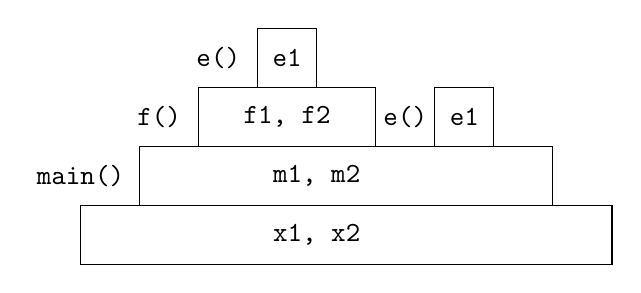
\begin{tikzpicture}
        \draw (0, 0) -- (6.75, 0)
            -- (6.75, 0.75)
            -- (0, 0.75)
            -- cycle;
        \node at (3, 0.375) {\texttt{x1, x2}};
        
        \draw (0.75, 0.75) -- (6, 0.75)
            -- (6, 1.5)
            -- (0.75, 1.5)
            -- cycle;
        \node at (3, 1.125) {\texttt{m1, m2}};
        \node at (0, 1.125) {\texttt{main()}};
        
        \draw (1.5, 1.5) -- (3.75, 1.5)
            -- (3.75, 2.25)
            -- (1.5, 2.25)
            -- cycle;
        \node at (2.625, 1.875) {\texttt{f1, f2}};
        \node at (1, 1.875) {\texttt{f()}};
        
        \draw (2.25, 2.25) -- (3, 2.25)
            -- (3, 3)
            -- (2.25, 3)
            -- cycle;
        \node at (2.625, 2.625) {\texttt{e1}};
        \node at (1.75, 2.625) {\texttt{e()}};
        
        \draw (4.5, 1.5) -- (5.25, 1.5)
            -- (5.25, 2.25)
            -- (4.5, 2.25)
            -- cycle;
        \node at (4.875, 1.875) {\texttt{e1}};
        \node at (4.125, 1.875) {\texttt{e()}};
    \end{tikzpicture}
\end{figure}
\noindent Global and local variable's lifetimes are nested. They cannot overlap.

Next, we consider a recursive program.
\begin{lstlisting}[language=C]
void main() {
    float m;
    // ..
    r(3);
}

void r(int n) {
    int i;
    if (n > 1) {
        // ..
        r(n-1);
    }
}
\end{lstlisting}
The following is the lifetime of the local variables.
\begin{figure}[H]
    \centering
    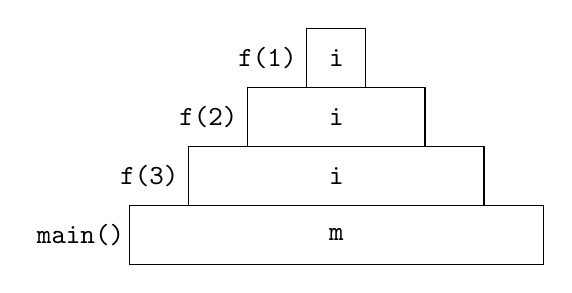
\begin{tikzpicture}
        \draw (0, 0) -- (5.25, 0)
            -- (5.25, 0.75)
            -- (0, 0.75)
            -- cycle;
        \node at (2.625, 0.375) {\texttt{m}};
        \node at (-0.625, 0.375) {\texttt{main()}};
        
        \draw (0.75, 0.75) -- (4.5, 0.75)
            -- (4.5, 1.5)
            -- (0.75, 1.5)
            -- cycle;
        \node at (2.625, 1.125) {\texttt{i}};
        \node at (0.25, 1.125) {\texttt{f(3)}};
        
        \draw (1.5, 1.5) -- (3.75, 1.5)
            -- (3.75, 2.25)
            -- (1.5, 2.25)
            -- cycle;
        \node at (2.625, 1.875) {\texttt{i}};
        \node at (1, 1.875) {\texttt{f(2)}};
        
        \draw (2.25, 2.25) -- (3, 2.25)
            -- (3, 3)
            -- (2.25, 3)
            -- cycle;
        \node at (2.625, 2.625) {\texttt{i}};
        \node at (1.75, 2.625) {\texttt{f(1)}};
    \end{tikzpicture}
\end{figure}
\noindent A local variable of a recursive procedure/function has several nested lifetimes.

Now, we consider heap variables. Consider the C program below.
\begin{lstlisting}[language=C]
struct IntNode {int elem; IntList succ;}
typedef struct IntNode * IntList;

IntList c (int h, IntList t) {
    IntList ns = (IntList) malloc (sizeof IntNode);
    ns -> element = h;
    ns -> succ = t;
    return ns;
}

void d (IntList ns) {
    ns -> succ = ns -> succc -> succ;
}

void main() {
    IntList l1, l2;
    l1 = c(3, c(5, c(7, NULL)));
    l2 = c(2, l1);
    d(l1);
}
\end{lstlisting}
The variables \texttt{l1} and \texttt{l2} are heap variables since they are initialised using the \texttt{malloc} keyword. The following is the heap representation of \texttt{l1} and \texttt{l2}.
\begin{figure}[H]
    \centering
    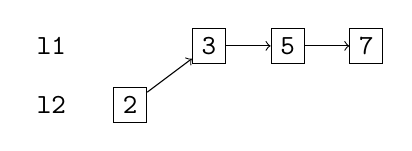
\begin{tikzpicture}
        \node[draw] (3) at (1, 0) {\texttt{3}};
        \node[draw] (5) at (2, 0) {\texttt{5}};
        \node[draw] (7) at (3, 0) {\texttt{7}};
        \node[draw] (2) at (0, -0.75) {\texttt{2}};

        \draw[->] (3) -- (5);
        \draw[->] (5) -- (7);
        \draw[->] (2) -- (3);

        \node at (-1, 0) {\texttt{l1}};
        \node at (-1, -0.75) {\texttt{l2}};
    \end{tikzpicture}
\end{figure}
\noindent After we call \texttt{d(l1)}, the state of \texttt{l1} and \texttt{l2} is the following.
\begin{figure}[H]
    \centering
    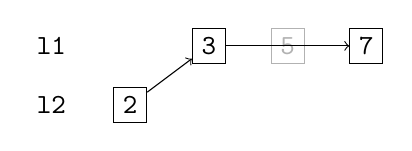
\begin{tikzpicture}
        \node[draw] (3) at (1, 0) {\texttt{3}};
        \node[draw, opacity=0.3] (5) at (2, 0) {\texttt{5}};
        \node[draw] (7) at (3, 0) {\texttt{7}};
        \node[draw] (2) at (0, -0.75) {\texttt{2}};

        \draw[->] (3) -- (7);
        \draw[->] (2) -- (3);

        \node at (-1, 0) {\texttt{l1}};
        \node at (-1, -0.75) {\texttt{l2}};
    \end{tikzpicture}
\end{figure}
\noindent As we can see, the value \texttt{5} is not reachable after calling \texttt{d}. 

The lifetime of the local and heap variables is given below.
\begin{figure}[H]
    \centering
    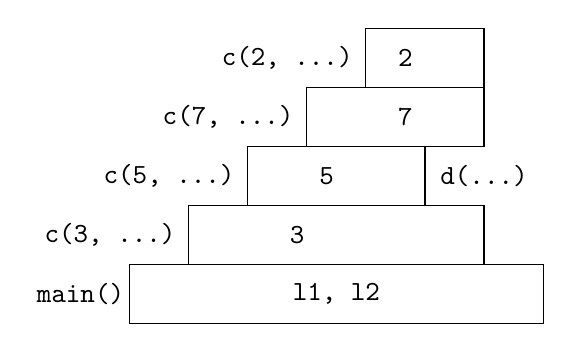
\begin{tikzpicture}
        \draw (0, 0) -- (5.25, 0)
            -- (5.25, 0.75)
            -- (0, 0.75)
            -- cycle;
        \node at (2.625, 0.375) {\texttt{l1, l2}};
        \node at (-0.625, 0.375) {\texttt{main()}};
        
        \draw (0.75, 0.75) -- (4.5, 0.75)
            -- (4.5, 1.5)
            -- (0.75, 1.5)
            -- cycle;
        \node at (2.125, 1.125) {\texttt{3}};
        \node at (-0.25, 1.125) {\texttt{c(3, ...)}};
        
        \draw (1.5, 1.5) -- (3.75, 1.5)
            -- (3.75, 2.25)
            -- (1.5, 2.25)
            -- cycle;
        \node at (2.5, 1.875) {\texttt{5}};
        \node at (0.5, 1.875) {\texttt{c(5, ...)}};
        \node at (4.5, 1.875) {\texttt{d(...)}};
        
        \draw (2.25, 2.25) -- (4.5, 2.25)
            -- (4.5, 3)
            -- (2.25, 3)
            -- cycle;
        \node at (3.5, 2.625) {\texttt{7}};
        \node at (1.25, 2.625) {\texttt{c(7, ...)}};
        
        \draw (3, 3) -- (4.5, 3)
            -- (4.5, 3.75)
            -- (3, 3.75)
            -- cycle;
        \node at (3.5, 3.375) {\texttt{2}};
        \node at (2, 3.375) {\texttt{c(2, ...)}};
    \end{tikzpicture}
\end{figure}
\noindent The lifetime of heap variables can overlap each other, and other local/global variable's lifetimes.

An allocator is an operation that creates a heap variable, yielding a pointer to the heap variable. For example, in C, the function \texttt{malloc} is the allocator, and in Java, an expression of the form \texttt{new C(..)} is an allocator. A deallocator is an operation that explicitly destroys a designated heap variable. For example, in C, the function \texttt{free} is the deallocator. Java does not have a deallocator.

A heap variable remains reachable as long as it can be accessed by following pointers from a local or a global variable. A heap variable's lifetime extends from its creation until:
\begin{itemize}
    \item it is destroyed by a deallocator,
    \item it becomes unreachable, or
    \item the program terminates.
\end{itemize}

A pointer is a reference to a particular variable. A pointer's referent is the variable to which it refers. A null pointer is a special pointer value that has no referent. A pointer is essentially the address of its referent in the store. However, each pointer also has a type, and the type of a pointer allows us to infer the type of its referent.

Pointers and heap variables can be used to represent recursive variables such as lists and trees. But, the pointer itself is a low-level concept. Manipulation of pointers is notoriously error-prone and hard to understand. For example, the C assignment \texttt{p -> succ = q;} appears to manipulate a list, but which list? Also,
\begin{itemize}
    \item Does it delete nodes from the list?
    \item Does it stitch together parts of two different lists?
    \item Does it introduce a cycle?
\end{itemize}

A dangling pointer is a pointer to a variable that has been destroyed. Dangling pointers arise when
\begin{itemize}
    \item a pointer to a heap variable still exists after the heap variable is destroyed by a deallocator
    \item a pointer to a local variable still exists at exit from the block in which the local variable was declared
\end{itemize}
A deallocator immediately destroys a heap variable. All existing pointers to that heap variable then become dangling pointers. For this reason, deallocators are inherently unsafe.

This means that C is somewhat unsafe and Java is safe. After a heap variable is destroyed in C, pointers to it might still exist. The same is true for local variables after we have exited their block. Java has no deallocator, so pointers to local variables cannot be obtained.

Now, consider the following C code.
\begin{lstlisting}[language=C]
struct Date {int y, m, d;}
typedef Date * DatePtr;

// date1 points to a newly-allocated heap node
DatePtr date1 = (DatePtr) malloc (sizeof Date);
date1->y = 2022;
date1->m = 1;
date1->d = 1;

// date2 points to the same heap variable
DatePtr date2 = date1;

// deallocates that heap variable- date1 and date2 now contain 
// dangling pointers
free(date2);

// behaves unpredictably
printf("%d4", date1->y);
date2->y = 2009;
\end{lstlisting}

A command (often called a statement) is a program construct that will be executed to update variables. Commands are characteristic of imperative and object-oriented PLs. Simple commands include:
\begin{itemize}
    \item A skip command is a command that does nothing.
    \item An assignment command is a command that uses a value to update a variable.
    \item A procedure call is a command that calls a proper procedure with argument(s). Its net effect is to update some variables.
\end{itemize}
Compound commands include:
\begin{itemize}
    \item A sequential command is a command that executes its sub-commands in sequence.
    \item A conditional command is a command that chooses one of its sub-commands to execute.
    \item An iterative command is a command that executes it sub-command repeatedly. This may be definite iteration, where the number of repetitions is known in advance, or an indefinite iteration, where the number is not known.
    \item A block command is a command that contains declarations of local variables.
\end{itemize}
Below are some examples in Java.
\begin{lstlisting}[language=Java]
// single assignment
m = n + 1;

// multiple assignment
m = n = 0;

// assignment with a binary operator
m += 7;
n /= b;

// if command
if (x > y) {
    System.out.println(x);
} else {
    System.out.println(y);
}

// switch command
Date today = ...;
switch (today.m) {
    case 1:
        System.out.println("JAN");
        break;
    ...
    case 12:
        System.out.println("DEC");
        break;
}

// while command
Date[] dates;
// ...
int i = 0;
while (i < dates.length) {
    System.out.println(dates[i]);
    i++;
}

// for command
for (int i = 0; i < dates.length; i++) {
    System.out.println(dates[i]);
}

// block command
if (x > y) {
    int z = x;
    x = y;
    y = z;
}
\end{lstlisting}

The primary purpose of evaluating an expression is to yield a value. In most imperative and object-oriented PLs, evaluating expressions can also update variables. These are side effects. In C and Java, the body of a function is a command. If that command updates a global or a heap variable, calling the function has side effects. In C and Java, assignments are expressions with side effects- \texttt{V = E} stores the value of \texttt{E} in \texttt{V}, as well as yielding that value.

The C function \texttt{getchar(fp)} reads a character and updates the file variable \texttt{fp} points to. So, the following C code is correct.
\begin{lstlisting}[language=C]
char ch;
while ((ch = getchar(fp)) != NULL) {
    putchar(ch);
}
\end{lstlisting}
On the other hand, the following C code is incorrect.
\begin{lstlisting}[language=C]
enum Gender {FEMALE, MALE};
Gender g;
if (getchar(fp) == "F") {
    g = FEMALE;
} else if (getchar(fp) = "M") {
    g = MALE;
}
\end{lstlisting}
\noindent This is wrong since the second invocation of \texttt{getchar(fp)} has moved past the character.
\newpage

\section{Bindings and Scope}
The meaning of an expression/command depends on the declarations of any identifiers used. A binding is a fixed association between an identifier and an entity (such as a value, variable or procedure). An environment (or namespace) is a set of bindings.

Each declaration produces some bindings which are added to the surrounding environment. Each expression/command is interpreted in a particular environment. Every identifier used in the expression/command have a binding in that environment.

The following is a C program outline, showing the environments for the two functions.
\begin{lstlisting}[language=C]
extern int z;
extern const float c = 3.0e6;

void f() {
    // ..

    // ENVIRONMENT:
        // c -> the FLOAT value 3 X 10^6
        // f -> a VOID -> VOID function
        // g -> a FLOAT -> VOID function
        // z -> an INT global variable
}

void g (float x) {
    char c;
    int i;
    // ..
    
    // ENVIRONMENT:
        // c -> a CHAR local variable
        // f -> a VOID -> VOID function
        // g -> a FLOAT -> VOID function
        // i -> an INT local variable
        // x -> a FLOAT local variable
        // z -> an INT global variable
}
\end{lstlisting}

The scope of a declaration (or of a binding) is the portion of the program text over which it has effect. In some early PLs, the scope of every declaration was the whole program. In modern PLs, the scope of each declaration is controlled by the program's block structure.

A block is a program construct that delimits the scope of any declarations within it. Each PL has its own forms of blocks:
\begin{itemize}
    \item In C, block commands (\texttt{\{ ... \}}), function bodies and compilation units are used;
    \item In Java, block commands (\texttt{\{ ... \}}), method bodies and class declarations are used;
    \item In Haskell, block expressions (\texttt{let ... in ...}), function bodies and modules are used.
\end{itemize}
A PL's block structure is the way in which blocks are arranged in the program text.

Some PLs such as Cobol have monolithic block structure- the whole program is a single block. The scope of every declaration is the whole program. This is depicted in the figure below.
\begin{figure}[H]
    \centering
    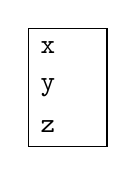
\begin{tikzpicture}
        \draw (0, 0) -- (0, 1.5)
            -- (1, 1.5)
            -- (1, 0)
            -- cycle;

        \node at (0.25, 1.25) {\texttt{x}};
        \node at (0.25, 0.75) {\texttt{y}};
        \node at (0.25, 0.25) {\texttt{z}};
    \end{tikzpicture}
\end{figure}

Some PLs such as Fortran have flat block structure- the program is partitioned into blocks, but these blocks may not contain inner blocks. This is depicted in the figure below.
\begin{figure}[H]
    \centering
    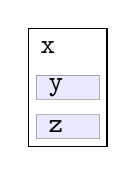
\begin{tikzpicture}
        \draw (0, 0) -- (0, 1.5)
            -- (1, 1.5)
            -- (1, 0)
            -- cycle;
            
        \draw[fill=blue!30, opacity=0.3] (0.1, 0.1) -- (0.1, 0.4)
            -- (0.9, 0.4)
            -- (0.9, 0.1)
            -- cycle;
        
        \draw[fill=blue!30, opacity=0.3] (0.1, 0.6) -- (0.1, 0.9)
            -- (0.9, 0.9)
            -- (0.9, 0.6)
            -- cycle;

        \node at (0.25, 1.25) {\texttt{x}};
        \node at (0.35, 0.75) {\texttt{y}};
        \node at (0.35, 0.25) {\texttt{z}};
    \end{tikzpicture}
\end{figure}

Modern PLs have nested block structure- blocks may be nested freely within other blocks. This is depicted in the figure below.
\begin{figure}[H]
    \centering
    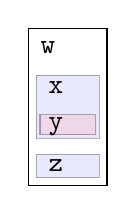
\begin{tikzpicture}
        \draw (0, 0) -- (0, 2)
            -- (1, 2)
            -- (1, 0)
            -- cycle;
            
        \draw[fill=blue!30, opacity=0.3] (0.1, 0.1) -- (0.1, 0.4)
            -- (0.9, 0.4)
            -- (0.9, 0.1)
            -- cycle;
        
        \draw[fill=blue!30, opacity=0.3] (0.1, 0.6) -- (0.1, 1.4)
            -- (0.9, 1.4)
            -- (0.9, 0.6)
            -- cycle;
        
        \draw[fill=red!30, opacity=0.3] (0.15, 0.65) -- (0.15, 0.9)
            -- (0.85, 0.9)
            -- (0.85, 0.65)
            -- cycle;

        \node at (0.25, 1.75) {\texttt{w}};
        \node at (0.35, 1.25) {\texttt{x}};
        \node at (0.35, 0.75) {\texttt{y}};
        \node at (0.35, 0.25) {\texttt{z}};
    \end{tikzpicture}
\end{figure}
\noindent With nested block structure, the scope of a declaration excludes any inner block whether the same identifier is declared.

For example, C has a flat block structure for functions, but nested block structure for variables. 
% This is depicted in the figure below.
% TODO: Add image
Having a flat block structure for functions means that we cannot declare functions within functions, but that they can be accessed from anywhere within the program.

A binding occurrence of identifier $I$ is an occurrence of $I$ where $I$ is bound to some entity $e$. An applied occurrence of identifier $I$ is an occurrence of $I$ where use is made of the entity $e$ to which $I$ is bound. If the PL is statically scoped, every applied occurrence of $I$ should correspond to exactly one binding occurrence of $I$. Below we have a C program, with binding occurrences and applied occurrences.
% TODO: ADD IMAGE
For each applied occurrence, there is one binding occurrence.

A PL is statically scoped if the body of a procedure is executed in the environment of the procedure definition. Then, we can decide at compile-time which binding occurrence of an identifier corresponds to a given applied occurrence. 

A PL is dynamically scoped if the body of a procedure is executed in the environment of the procedure call site. Then, we cannot decide until runtime which occurrence of an identifier corresponds to a given applied occurrence, since the environment may vary from one call site to another.

The following is a program in C, a statically scoped language.
% TODO: Add diagram
In a hypothetical, dynamically scoped PL, we get the following situation.
% TODO: Add diagram

Dynamic scoping fits badly with static typing. Nearly all PLs are statically scoped. Only a few PLs, such as Smalltalk and Lisp are dynamically scoped.

A declaration is a program construct that will be elaborated to produce binding(s). A declaration may also have side effects, such as creating a variable. A definition is a declaration whose only effect is to produce binding(s). It has no side effects.

Simple declarations include:
\begin{itemize}
    \item A type declaration binds an identifier to an existing or new type.
    \item A constant definition binds an identifier to a value, possible after computation.
    \item A variable declaration binds an identifier to a newly-created variable.
    \item A procedure definition binds an identifier to a procedure.
\end{itemize}

A recursive definition is one that uses the bindings it produces itself. In almost all PLs, recursion is restricted to type (or class) declarations and procedure (or method) declarations. 

An example below is given of a recursive Java class, with a recursive method.
\begin{lstlisting}[language=Java]
class IntList {
    int head;
    IntList tail;
    
    static int length(IntList list) {
        if (list == null) {
            return 0;
        } else {
            return 1 + length(list.tail);
        }
    }
}
\end{lstlisting}
C struct type declarations may be recursive, but only via pointers. Also, C function definitions may be recursive. Below is the C version of the class \texttt{IntList} above.
\begin{lstlisting}[language=C]
struct IntList {
    int head;
    struct IntList * tail;
}

int length(IntList * list) {
    if (list == NULL) {
        return 0;
    } else {
        return 1 + length(list->tail);
    }
}
\end{lstlisting}
\newpage

\section{Abstraction}
In programming, abstraction means the distinction between what a program unit does and how it performs the task. This supports a separation of concerns between the implementor (i.e. who codes the program unit) and the application programmer (i.e. who uses it). Program units include procedures, packages, classes and generic packages.

\subsection{Procedural Abstraction}
A proper procedure (or just procedure) embodies a command to be executed. A procedure call is a command. It causes the procedure's body to be executed. It results in the update of some variables.

A function procedure (or just function) embodies an expression to be evaluated. A function call is an expression. It causes the function's body to be evaluated. It results in a value (which is returned by the function).

Imperative PLs usually support both procedures and functions. For example, in Pascal and Ada, procedures and functions are syntatically distinct. However, in C and Java, the only distinction is that a procedure's result type is \texttt{VOID}. Functional PLs only support functions. Object-oriented PLs also support procedures as methods. A static method is a procedure exported by a class. An instance method is a procedure attached to an object.

The following is a procedure in C.
\begin{lstlisting}[language=C]
void print(Date date) {
    int y = date.y,
        m = date.m,
        d = date.d;
    printf("%d4-%d2-%d2", y, m, d);
}
\end{lstlisting}
The procedure body is a block command. The execution of the procedure results in the variables \texttt{y}, \texttt{m} and \texttt{d} being created.

The following is a function in Haskell.
\begin{lstlisting}[language=Haskell]
power   ::  (Float, Int) -> Float
power (b, n) =
    if n == 0
    then 1.0
    else b * power(b, n-1)
\end{lstlisting}
The body of the function is an expression. The following is the same function in C.
\begin{lstlisting}[language=C]
float power(float b, float n) {
    float p = 1;
    while (n > 0) {
        p *= b;
        n--;
    }
    return p;
}
\end{lstlisting}
Here, the body of the function is still a block command.

In most imperative and object-oriented PLs, the function's body is syntatically a block command. This is executed until a return determines the function's result. This means that the full expressive power is available to define a function (e.g. instantiate variables). However, this is a roundabout way to compute a result. In fact, a return might never be executed (e.g. because of an infinite loop). Moreover, side effects are possible.

In functional PLs, the function's body is syntatically an expression. This is evaluated to yield the function's result. This means that the design is simple and natural. However, the expressive power of the PL is limited. This can be remedied by allowing conditional and iterative expressions, nonetheless.

An argument is a value (or another entity) that is passed to a procedure. An actual parameter is an expression that yields an argument. A formal parameter is an identifier through which a procedure can access an argument. We can pass the following as arguments:
\begin{itemize}
    \item values,
    \item variables, or pointers to variables, and
    \item procedures, or pointers to procedures.
\end{itemize}

A parameter mechanism is a means by which a formal parameter provides access to the corresponding argument. Different PLs support a variety of parameter mechanisms: value, result, value-result, constant, variable, procedural and functional parameters. These can all be understood in terms of two underlying concepts: copy parameter mechanisms and reference parameter mechanisms.

With a copy parameter mechanism, a value is copied into and/or out of a procedure. A formal parameter is bound to a local variable of the procedure. A value is copied into that local variable on calling the procedure. A value is copied into that local variable on calling the procedure. The value can also be copied out of that local variable to an argument variable on return. There are 2 copy parameter mechanisms- copy in and copy out parameter.

In copy-in parameter (or value parameter), the argument is a value. On call, a local variable is created and initialised with the argument value. On return, the local variable is destroyed.

In copy-out parameter (or result parameter), the argument is a variable. On call, a local variable is created but not initialised. On return, the local variable's final value is assigned to the argument variable, then the local variable is destroyed.

The following is some functions in C.
\begin{lstlisting}[language=C]
void print(Date date) {
    printf("%d-%d-%d", date.y, date.m, date.d);
}

void main() {
    Date today = {2022, 3, 7};
    print(today);
}
\end{lstlisting}
At line 1, the local variable \texttt{date} is initialised to the argument value. At line 7, the argument value is \texttt{\{2022, 3, 7\}}.

With a reference parameter mechanism, the formal parameter is a reference to the argument. The formal parameter FP is bound to a reference to the argument. Every accessed to FP is an indirect access to the argument. There are 3 principal reference parameter mechanisms- constant, variable and procedural parameter.

In a constant parameter mechanism, the argument is a value. So, any inspection of the FP is an indirect inspection of the argument value. In a variable parameter mechanism, the argument is a variable. So, any access (inspection or update) of the FP is an indirect access of the argument variable. In a procedural parameter mechanism, the argument is a procedure. So, any call to the FP is an indirect call to the argument procedure.

The following is some methods in Java.
\begin{lstlisting}[language=Java]
public void print(Date date) {
    System.out.println(date.y & "-" date.m & "-" & data.d);
}

public static void main() {
    Date today = new Date(2022, 3, 7);
    print(today);
}
\end{lstlisting}
At line 1, the local variable \texttt{date} is a reference to the argument object. At line 7, the argument is the object to which \texttt{today} refers. Java supports copy-in parameter mechanism for primitive types. Also, Java supports the reference parameter mechanism for object types.

\subsection{Data abstraction}
A package (or module) is a named group of components declared for a common purpose. These components may be types, constants, variables, procedures, inner packages, etc. The meaning of a package is the set of bindings exported by the package. These are often called the packages's application program interface (API).

An example is given below in Python.
\begin{lstlisting}[language=python]
words = [...]

def contains(word):
    global words
    return word in words

def add(word):
    global words
    if word not in words:
        words += [word]
\end{lstlisting}
This module's API contains the variable \texttt{words} and the functions \texttt{contains} and \texttt{add}.

Some of the components of a program unit (package/class) may be private. This is called encapsulation. There are many levels of privacy, as given below.
\begin{itemize}
    \item A component is private if it is visible only inside the program unit.
    \item A component is protected if it is visible only inside the program unit and certain other program units.
    \item A component is public if it is visible to application code outside the program unit.
\end{itemize}
A program unit API consists of its public bindings only.

Most PLs (such as Ada, java, Haskell) allow individual components of a program unit to be specified as private, protected or public. Python has a convention that components whose names start with "\_" are private, and anything else is public. This is not enforced by the Python compiler.

In Java, the components of a package are classes and inner packages. Package components are added incrementally. The following is the outline of a class declaration within a package.
\begin{lstlisting}[language=java]
package sprockets;

import widgets.*;

public class C {
    ...
}
\end{lstlisting}
At line 1, we declare that the class \texttt{C} is a component of the package \texttt{sprockets}. At line 3, we declare that the class \texttt{C} uses public components of the pakcage \texttt{widgets}.

An object is a tagged tuple of variable components (instance variables), equipped with operations that access these instance variables. A constructor is an operation that initialises a newly created object. An instance method is an operation that inspects and/or updates an existing object of the class. That object (called the receiver object) is determined by the method call. A class is a set of similar objects. All objects of a given class have similar instance variables, and are equipped with the same operations.

A Java class declaration declares its instance variables and defines its constructors and instance methods. It also specifies whether each of these is private, protected or public. A Java instance method call has the form \texttt{O.M(...)}. The expression \texttt{O} yields the receiver object. \texttt{M} is the name of the instance method to be called. The call executes the method body, with \texttt{this} bound to the receiver object \texttt{O}.

We illustrate this with an example.
\begin{lstlisting}[language=java]
class Dict {
    private int size;
    private String[] words;

    public Dict(int capacity) {
        ...
    }

    public void add (String w) {
        if (!this.contains(w)) {
            this.words[this.size++] = w;
        }
    }

    public boolean contains (String w) {
        ...
    }
}
\end{lstlisting}
A possible application code is the following.
\begin{lstlisting}[language=java]
Dict mainDict = new Dict(10000);
Dict userDict = new Dict(100);
...
if (!mainDict.contains(currentWord) && !userDict.contains(currentWord)) {
    userDict.add(currentWord);
}
\end{lstlisting}
It is not however possible to do the following.
\begin{lstlisting}[language=java]
userDict.size = 0;
System.out.println(userDict.words[0]);
\end{lstlisting}
This is because the two instance variables are private.

If $C'$ is a subclass of $C$ (or $C$ is a superclass of $C'$), then $C'$ is a set of objects that are similar to one another, but richer than the objects of class $C$. In particular, an object of class $C'$ has all the instance variables of an object of class $C$. But, it can have extra instance variables. Similarly, an object of class $C'$ is equipped with all the instance methods of class $C$. But, it can also override some of them, and there might be extra instance methods.

By default, a subclass inherits (or shares) it superclass' instance methods. Alternatively, a subclass may override some of its superclass' instance methods by providing more specialised versions of these methods.

To illustrate this, consider the following class in Java.
\begin{lstlisting}[language=java]
class Shape {
    protected float x, y;

    public Shape() {
        this.x = 0.0;
        this.y = 0.0;
    }

    public final void move(float dx, float dy) {
        this.x += dx;
        this.y += dy;
    }

    // draw a point at (x, y)
    public void draw() {
        ...
    }
}
\end{lstlisting}
We define the subclass \texttt{Circle}.
\begin{lstlisting}[language=java]
class Circle extends Shape {
    private float r;

    public Circle(float radius) {
        this.x = 0;
        this.y = 0;
        this.r = radius;
    }

    // draw a circle at (x, y) of radius r
    @override
    public void draw() {
        ...
    }

    public float diameter() {
        return 2.0 * r;
    }
}
\end{lstlisting}
A possible application code is given below.
\begin{lstlisting}[language=java]
Shape s = new Shape();
Circle c = new Circle(10.0);
s.move(12.0, 5.0);
c.move(3.0, 4.0);

System.out.println(c.diameter());
s.draw();
c.draw();

s = c;
s.draw();
\end{lstlisting}
At line 7, we draw a point at \texttt{(12, 5)}. At line 8, we draw a circle at \texttt{(3, 4)} with radius \texttt{10}. We draw the same circle at line 11. This is dynamic dispatch- we draw a circle since \texttt{s} is a \texttt{Circle}.

Each instance method of a class $C$ is inherited by the subclass $C'$, unless it is overriden by $C'$. The overriding method in class $C'$ has the same name and type as the original method in class $C$. Most object-oriented PLs allow the programmer to specify whether an instance method is \texttt{virtual} (may be overriden) or not. For example, in C++, an instance method specified by \texttt{virtual} may be overriden. In Java, an instance method specified by \texttt{final} cannot be overriden.

In every object-oriented PL, a variable of type $C$ may refer to an object of any subclass of $C$. If a method $M$ is virtual, then the method call \texttt{O.M} entails dynamic dispatch. The compiler infers the type of $O$ as class $C$. It then checks that class $C$ is equipped with an instance method named $M$ of the appropriate type. At run-time, however, it might turn out that the receiver object is of class $C'$, a subclass of $C$. The receiver object's tag is used to determine its actual class, and hence determine which of the methods named $M$ is to be called.

An object-oriented PL supports single inheritance if each class has at most one superclass. Single inheritance gives rise to a hierarchy of class. Single inheritance is supported by most object-oriented PLs. 

Multiple inheritance allows each class to have any number of superclasses. It is supported by C++. Multiple inheritance gives rise to both conceptual and implementation problems. For example, if both the superclasses override a method, then which version should be used within the subclass. To mitigate this, we might require the subclass to override the method, or use a priority system with the superclasses.

\subsection{Generic abstraction}
A program unit is generic if it is parameterised with respect to a type on which it depends. Many reusable program units (e.g. stack, list) are naturally generic. Generic program units include: generic packages, generic classes and generic procedures.

In Java, a generic class GC is parameterised with respect to a type $T$ on which it depends.
\begin{lstlisting}[language=Java]
class GC<T> {
    ...
}
\end{lstlisting}
The generic class must be instantiated by substituting a type argument $A$ for the type parameter $T$, i.e. \texttt{GC<A>}. This instantiation generates an ordinary class.

The following is a declaration of a generic class.
\begin{lstlisting}[language=Java]
class List<T> {
    private static final cap = 100;
    private int size;
    private T[] elems;

    public List() {
        size = 0;
        elems = (T[]) new Object[cap];
    }

    public void add(T elem) {
        elems[size++] = elem;
    }
}
\end{lstlisting}
We can then make use of this class as follows.
\begin{lstlisting}[language=Java]
public static void main() {
    List<String> sentence;
    sentence = new List<String>();
    sentence.add("...");
}
\end{lstlisting}
In Java, the type argument must be a class, not a primitive type.

Java also supports generic interfaces, such as \texttt{Comparable}.
\begin{lstlisting}[language=Java]
interface Comparable<T> {
    public int compareTo(T that);
}
\end{lstlisting}
If a class $C$ is declared as implementing \texttt{Comparable<C>}, then $C$ must be equipped with a \texttt{compareTo} method that compares objects of type $C$.

Consider a generic class \texttt{GC<T>} that requires \texttt{T} to be equipped with some specific methods. Then, \texttt{T} may be specified as bounded by a class \texttt{C}.
\begin{lstlisting}[language=Java]
class GC<T extends C> {
    ...
}
\end{lstlisting}
\texttt{T} is known to be equipped with all the methods of \texttt{C}, so we can make use of them within this class. Now, the type argument must be a subclass of \texttt{C}. Alternatively, \texttt{T} may be specified as bounded by an interface \texttt{I}. Moreover, \texttt{GC<T>} actually stands for \texttt{GC<T extends Object>}. The type argument must be a subclass of \texttt{Object}, which applies to all the classes.

\end{document}
